\chapter{Soluci\'on Conceptual}
\newpage
\section{Diagn\'ostico de la situaci\'on actual}
\subsection{Situaci\'on Actual}

En la actualidad existen distintas tecnolog\'ias en cuanto a las mascotas que se est\'an de\-sa\-rro\-llan\-do en el mundo. A pesar de ello, es posible catalogarlas en dos grandes grupos:

\begin{itemize}
\item Mascotas Virtuales
\item Mascotas Rob\'oticas
\end{itemize}

En cuanto a las Mascotas Virtuales, estas corresponden a aquellas que no poseen un cuerpo real con el cual interactuar y su medio de presentaci\'on corresponde a un dispositivo (dise\~nado para ese \'unico prop\'osito o para varios) que, a trav\'es de botones o instrucciones dadas por medio de una pantalla, interact\'ua con la mascota correspondiente.

Por otro lado, las Mascotas Rob\'oticas poseen un nivel de complejidad mayor; esto debido, en gran medida, a la presencia de un cuerpo f\'isico con el cual el usuario puede interactuar. La mascota no solo debe saber responder a diferentes est\'imulos del entorno, sino que incluso el cuerpo mismo debe poder mostrar las reacciones correspondientes (a pesar de que esto no es necesario que ocurra con todo el cuerpo del robot).

Finalmente, se destacan algunos productos correspondientes a ambas \'areas:
\subsubsection{ Mascotas Virtuales}
  \begin{enumerate}
  \item \emph{Pou},\footnote{\url{https://play.google.com/store/apps/details?id=me.pou.app/}} una aplicaci\'on para Android, que posee minijuegos sencillos, adem\'as de las caracter\'isticas naturales de unas mascota (como alimentarlo o ba\~narlo, por ejemplo). Tambi\'en permite la interacci\'on con las mascotas de otros usuarios.
  \item \emph{Mou},\footnote{\url{http://www.windowsphone.com/es-cl/store/app/mou/c032d62c-7f6a-4538-8150-f77034dcf335/}} aplicaci\'on de Windows Phone similar a Pou, aunque posee con una cantidad de juegos y acciones posibles, m\'as limitado que este.
  \item \emph{Tamagotchi},\footnote{\url{http://tamagotchilife.com/}} dispositivo port\'atil que simular una mascota, la cual debe cuidarse y criarse. Tambi\'en tiene la habilidad de interactuar con otros dispositivos en sus versiones m\'as recientes.
  \item \emph{Pet Society},\footnote{\url{https://www.facebook.com/petsociety/info}} conocida aplicaci\'on de Facebook en la que se cuida y juega con una mascota, adem\'as de posibilitar la interacci\'on con las mascotas de la lista de contactos del usuario que utilizan dicha aplicaci\'on.
  \item \emph{Petz},\footnote{\url{http://petz.uk.ubi.com/}} saga de juegos para las consolas Nintendo en la cual el usuario se encarga de cuidar perros y gatos, los cuales (para el caso de las consolas port\'atiles) pueden interactuar con otros.
  \end{enumerate}
\subsubsection{Mascotas Rob\'oticas}
  \begin{enumerate}
  \item \emph{Furby},\footnote{\url{http://www.furby.es/es_ES/}} famosas en los 2000, los cuales era posible alimentar e interactuaban con otros de su misma clase.
  \item \emph{FurReal Friends},\footnote{\url{http://www.hasbro.com/furreal/en_US/}} mascotas rob\'oticas dise\~nadas para ni\~nas, las cuales reaccionan a caricias y realizan gestos similares a las de una mascota real.
  \item \emph{Aibo},\footnote{\url{http://www.sony-aibo.co.uk/}} mascota fabricada por Sony. Simula un perro y posee sensores que le evitan chocar con objetos, una cola que funciona como antena adem\'as de ``sentido del tacto'' y un simulador de inteligencia artificial. Es utilizado por universidades e institutos para realizar estudios de inteligencia artificial.
  \end{enumerate}


\subsection{Identificaci\'on de problemas y deficiencias}

Si bien el mundo de las mascotas virtuales ha tenido cambios desde sus or\'igenes, estos no han variado mucho respecto a su concepci\'on original, sino que su mayor cambio ha sido en la forma de realizar la interacci\'on con ellos, cambio que fue potenciado con la llegada de los dispositivos llamados ``\emph{touch}''.

En contraparte, el aumento en el nivel de tecnolog\'ia actual, y la disminuci\'on de tama\~no de procesadores y otros componentes electr\'onicos, ha permitido la llegada al mercado de mascotas rob\'oticas a precios accesibles, situaci\'on que habr\'ia sido imposible a\~nos antes. Adem\'as de esto, las nuevas tecnolog\'ias permiten agregarle mayores funcionalidades a los robots utilizados. De esta manera puede verse una gran diferencia entre \emph{Furby}, que tan s\'olo permit\'ia la identificaci\'on de ciertos patrones de voz y el movimiento de ojos y orejas, y \emph{Aibo}, que posee sensores de sonido, inteligencia artificial y sensores t\'actiles, lo que lo convierten en una mascota m\'as realista (adem\'as de tener un movimiento similar al de un perro real).

A pesar de que ambas tecnolog\'ias han avanzado, hay que destacar que no existe una forma de interactuar entre ellas, y su utilizaci\'on actual corresponde \'unicamente a potenciar la primera o la segunda. Dicha brecha corresponde a un problema en el uso de las mascotas virtuales, ya que es una potencialidad que podr\'ia ser aprovechable a futuro.

Cabe destacar, en todo caso, que la adopci\'on masiva de mascotas rob\'oticas es un tema de discusi\'on aparte, debido a la necesidad, de estas, de poder desenvolverse eficientemente en el medio al que sea llevado, lo cual requiere un alto nivel de tecnolog\'ia, lo cual redundar\'ia en un mayor costo para el usuario.

Omitiendo lo anterior, por caer fuera de nuestro rango de acci\'on, mezclar las tecnolog\'ias actuales en rob\'otica, junto con las correspondientes en el \'area de los dispositivos m\'oviles, para utilizar ambos en el desarrollo de mascotas virtuales se destaca como una de las grandes falencias, en la actualidad, en el uso de este tipo de aplicaciones. Es un nicho no explotado en el presente, y que podr\'ia ser de gran potencialidad, debido a la masificaci\'on que existe en estos momentos en el uso de dispositivos m\'oviles.

\newpage
\section{Caracterizaci\'on del cambio}
\subsection{Caracter\'isticas y potencialidades deseadas}

Se espera que el sistema a implementar posea y/o sea capaz de:
\begin{itemize}
\item {\bf Simular una mascota a trav\'es de un dispositivo m\'ovil, espec\'ificamente un smartphone, con SO Android};
\item {\bf Permitir la interacci\'on entre el usuario y la mascota virtual, por medio de los distintos elementos internos del smartphone} (como son la pantalla t\'actil, a\-ce\-le\-r\'o\-me\-tro, sensor de sonido, bater\'ia, entre otros);
\item {\bf Permitir la interacci\'on entre el usuario y el robot LEGO Mindstorms, por medio de los sensores disponibles para este} y
\item {\bf Permitir la interacci\'on entre el smartphone con SO Android y el robot LEGO Mindstorms, para la realizaci\'on de distintas actividades en cada uno de ellos}.
\end{itemize}

\subsection{Restricciones}

Para un buen desarrollo del proyecto, y de manera tal que cumpla con las caracter\'isticas y potencialidades anteriormente descritas, es necesario que \'este cumpla con las siguientes restricciones:
\begin{enumerate}
\item {\bf Sistema operativo (SO) del dispositivo m\'ovil a utilizar sea de f\'acil acceso, para facilitar la masificaci\'on del producto};
\item {\bf Bajo costo para la implementaci\'on del software};
\item {\bf Permitir que la aplicaci\'on funcione entre distintas versiones del SO};
\item {\bf Conectividad entre robot y Smartphone debe ser v\'ia Bluetooth};
\item {\bf Tiempo de desarrollo del proyecto limitado, es decir, con un m\'aximo de 1500 horas, aproximadamente, a distribuir entre los miembros del equipo}.
\item {\bf Alejamiento de unos de los integrantes para el segundo semestre del a\~no en curso.}
\end{enumerate}

\newpage
\section{An\'alisis de las alternativas de la soluci\'on}

Para poder ver otras posibles alternativas existentes, analizaremos seg\'un las distintas opciones existentes. Para esto se revisar\'an los dos aspectos m\'as importantes en todo el proyecto, como son el dispositivo m\'ovil a utilizar y el modelo rob\'otico. Estos se detallan a continuaci\'on.
\subsection{Respecto al dispositivo m\'ovil}
Corresponden a aquellos que se basan en SO del equipo. Descatan:
  \begin{enumerate}
  \item {\bf Basado en iOS}:\footnote{\url{http://www.apple.com/es/ios/}} Sistema de gran estabilidad y eficiencia. Destaca la alta llegada de las aplicaciones en la Store de Apple, y el alto control que se hace de estas en dicha plataforma para su publicaci\'on. Como contra, se puede destacar el bajo nivel de accesibilidad, adem\'as de la necesidad de equipos Mac para el desarrollo de software
  \item {\bf Basado en Windows Phone}:\footnote{\url{http://www.windowsphone.com/en-us/}} En cuanto a las ventajas, destaca la familiaridad y sencillez del mismo, adem\'as de la portabilidad de c\'odigo a los distintos dispositivos de Microsoft, e incluso a Mac OS X (por medio de Silverlight). Tambi\'en la presencia del Market de Windows. Punto en contra es su baja presencia en el mercado, adem\'as de que s\'olo la \'ultima versi\'on del mismo posee soporte para procesadores multin\'ucleo, adem\'as del costo de adquisici\'on de los equipos.
  \item {\bf Basado en Android}:\footnote{\url{http://www.android.com/}} Como puntos a favor, se puede encontrar una gran presencia en el mercado, adem\'as de una Store donde alojar aplicaciones. Por otro lado, tiene un nivel de acceso bajo en comparaci\'on con otros SO y la facilidad de desarrollar aplicaciones en distintos entornos (como pueden ser Windows o Linux). Punto en contra a destacar es la mala compatibilidad entre versiones, adem\'as del control de calidad presente \'unicamente para las \'ultimas versiones de Android. Cabe destacar que todos los miembros del equipo poseen dispositivos basados en Android.
  \end{enumerate}
\subsection{Respecto al modelo Rob\'otico}
 Corresponden a los que estan basados en estructuras f\'isicas. Principalmente se destacan:
  \begin{enumerate}
  \item {\bf Arduino}:\footnote{\url{http://www.arduino.cc/}} Es posible ver las grandes posibilidades que existen con este sistema. La posibilidad de crear modelos rob\'oticos de gran complejidad, adem\'as de la libertad de programaci\'on personalizada, donde est\'a la libertad de elecci\'on de como programar cada componente. Como punto en contra est\'a el que es necesario construir el equipo rob\'otico desde cero, utilizando servos para ciertos movimientos, motores.
\begin{figure}[H]
  \centering
  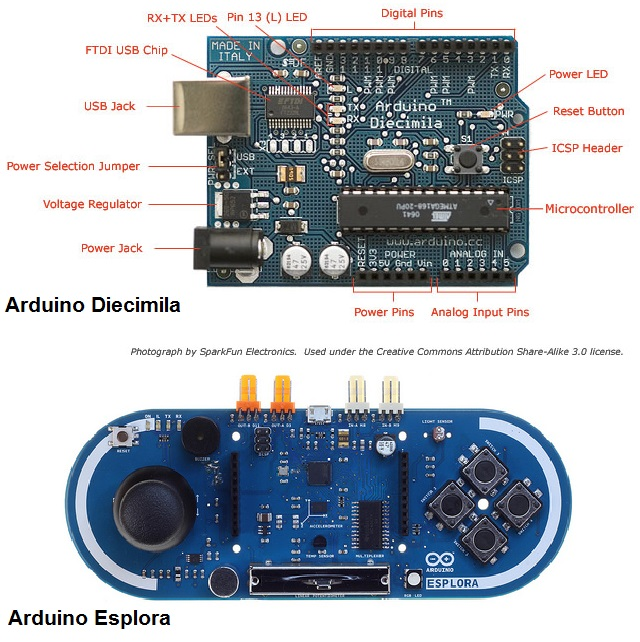
\includegraphics[scale=0.4]{Arduino.jpg}
  \caption[~Placas de Arduino]{Algunas de las placas de Arduino existentes en el mercado.}
  \label{fig:LegoMindstorms}
\end{figure}

  \item {\bf LEGO Mindstorms}:\footnote{\url{http://mindstorms.LEGO.com/en-us/default.aspx/}} Dentro de las fortalezas de este tipo de sistema, destaca su facilidad de armado y la predefinici\'on de muchos de sus sistemas, adem\'as de la versatilidad de funciones que es capaz de desarrollar. Al mismo tiempo, su alto costo y la restricci\'on del software necesario para desarrollar en \'el se destacan como sus mayores debilidades. Al mismo tiempo posee una baja curva de aprendizaje a la hora de programarlo; sin incluir que no es necesario saber de electr\'onica para su armado.
\begin{figure}[H]
  \centering
  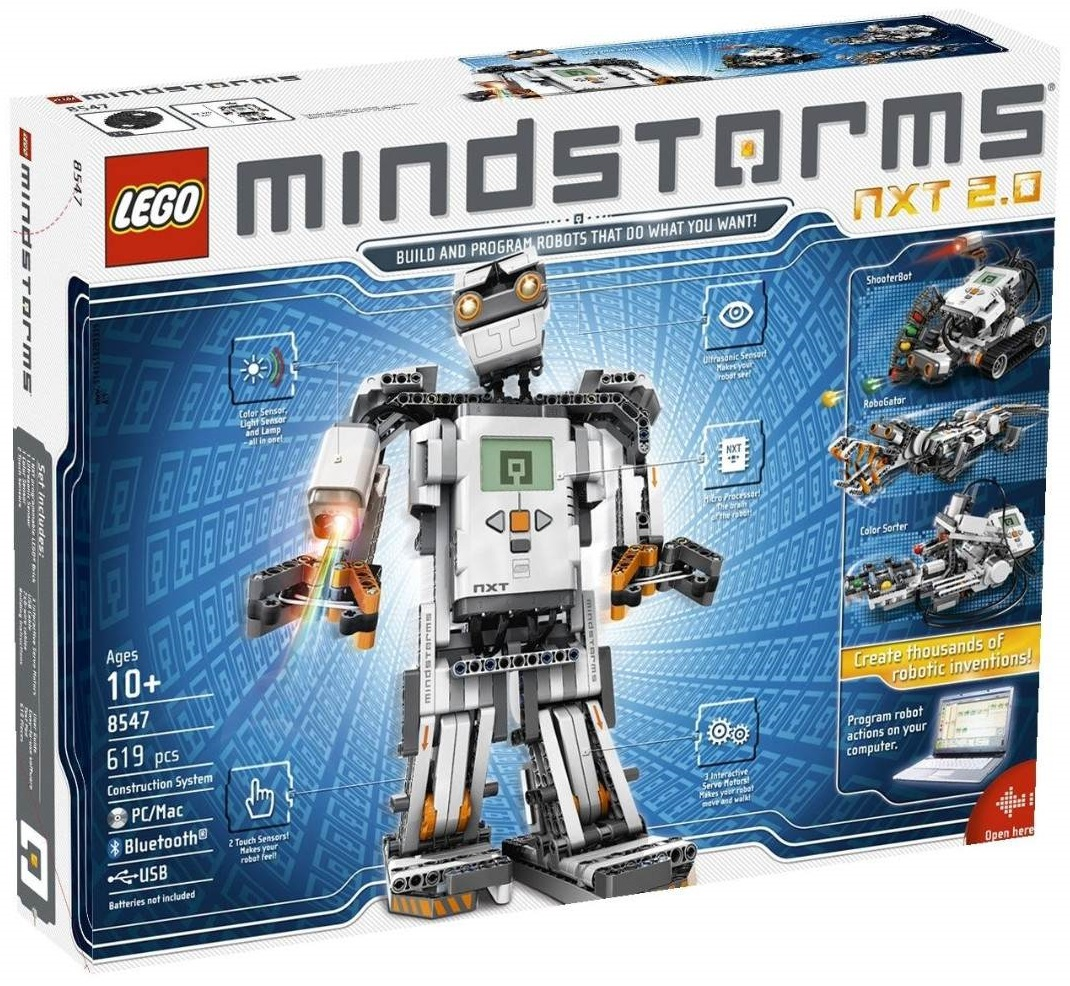
\includegraphics[scale=0.25]{LegoMindstorms.jpg}
  \caption[~LEGO Mindstorms]{Box de LEGO Mindstorms.}
  \label{fig:LegoMindstorms}
\end{figure}

  \end{enumerate}

\newpage
\section{Soluci\'on recomendada}

En base a todo lo expuesto con anterioridad, el enfoque del proyecto que se plantea, co\-rres\-pon\-de a la uni\'on de dos tecnolog\'ias, es decir, el uso de mascotas tanto en el \'ambito virtual como rob\'otico, permitiendo la interacci\'on del usuario por medio de estas dos plataformas. Para ello, se hace necesario poder identificar las tecnolog\'ias a utilizarse, en base a las restricciones planteadas.

Atendiendo a la restricci\'on n\'umero 5, referente al tiempo de duraci\'on del proyecto, la utilizaci\'on de Arduino o similares queda descartada, debido al alto impacto que tendr\'ia en el tiempo de duraci\'on de este. Dise\~nar y construir un robot con las caracter\'isticas requeridas, en cuanto a sensores, movimiento y comunicaci\'on, requiere una cantidad de tiempo y per\-so\-nal que exceder\'ia las restricciones de tiempo impuestas (ya que adem\'as del robot a utilizar, es necesaria la implementaci\'on del software correspondiente). En vista de ello, se har\'a utilizaci\'on de los robot LEGO Mindstorms, lo que disminuir\'a en gran medida el costo de tiempo para la construcci\'on del modelo rob\'otico, permitiendo adem\'as, una gama amplia de posibles dise\~nos de robots que puedan ser utilizados para el desarrollo del proyecto, debido a su gran versatilidad en la construcci\'on.

En cuanto a la restricci\'on n\'umero 4, esta queda solucionada inmediatamente con la selecci\'on de LEGO Mindstorms, debido a que es posible comunicar los NXT Intelligent Brick\footnote{\url{http://www.mathcs.org/robotics/nxt-java/building/nxt_intro.html/}} por medio de la tecnolog\'ia Bluetooth a los dispositivos m\'oviles. Por lo que no afecta en nada a la selecci\'on del modelo rob\'otico ya planteada. En cuanto al SO a utilizar, esta restricci\'on no ayuda en su determinaci\'on, ya que todos lo dispositivos m\'oviles, en la actualidad, cuentan con Bluetooth.

Respecto a la restricci\'on n\'umero 3, existen librer\'ias para tratar con la compatibilidad entre distintas versiones de los distintos SO existentes en el mercado, por lo que tampoco es determinante en la selecci\'on de la tecnolog\'ia m\'ovil a utilizar.

Finalmente, en respuesta a la restricci\'on n\'umero 2, que impone un bajo costo en el desarrollo del proyecto y en relaci\'on a la restricci\'on n\'umero 1, que habla sobre la facilidad de acceso de los dispositivos m\'oviles, se har\'a uso de SO Android. Lo anterior debido a que corresponde al SO con un mayor mercado en el \'ambito de los dispositivos m\'oviles (en contraste con Windows Mobile o iOS\cite{bib:Tendencias}\cite{bib:MobileDevices}) y, por otro lado, el acceso a desarrollo de aplicaciones no se encuentra limitado a SO determinados (como corresponde al caso iOS, que requiere equipos iMac para su elaboraci\'on, que poseen un costo de adquisici\'on alto).

En vista de lo expuesto con anterioridad, se reafirma el uso de SO Android en los dispositivos m\'oviles a utilizar, adem\'as de LEGO Mindstorms para los robots a dise\~nar durante el desarrollo del proyecto.
